\documentclass{uwstat572}

\usepackage{graphicx}
\usepackage{float}

%%\setlength{\oddsidemargin}{0.25in}
%%\setlength{\textwidth}{6in}
%%\setlength{\topmargin}{0.5in}
%%\setlength{\textheight}{9in}

\renewcommand{\baselinestretch}{1.5} 


\bibliographystyle{apalike}

\begin{document}
%%\maketitle

\begin{center}
  {\LARGE Statistical inference and computational efficiency for spatial infectious disease models with plantation data}\\\ \\
  {Nathan Welch \\ 
    Department of Statistics, University of Washington Seattle, WA, 98195, USA
  }
\end{center}

\begin{abstract}
This report examines the findings published in \textit{Statistical inference and computational efficiency for spatial infectious disease models with plantation data} \cite{Brown}. 
This paper aims conduct statistical inference on parameters associated with a simple individual level model. 
Model parameters are estimated using the Metropolis sampling algorithm; however, the computation burden created by fitting even a simple model leads to prohibitively long computation time. 
Statistical and computational methods to overcome the computing challenge are reviewed as a result. 
\end{abstract}

\section{Introduction}

Disease propagation modeling is an expansive and active area of mathematical research.
Statistical inference for parameters underlying these models is less mature.
\cite{Brown} set out to conduct statistical inference for a simple class of disease propagation models by estimating the risk that a susceptible individual contracts a disease from an infected member of the population. 
In these models, the risk of contracting the disease is modeled at the individual level rather than for the population as a whole. 
The goal is to formulate models that reflect changes in individual risk that correspond to the number of the infected individuals, their proximity to susceptible members of the population, and the duration a susceptible individuals  exposure to those infected. 
While this model is conceptually convenient, the computational complexity and limitations of algorithms capable of fitting such a model create significant challenges.
In \cite{Brown}, the authors appeal to standard likelihood methods and the Metropolis algorithm to estimate a simple ILM disease propagation model.
The emphasis on basic components like the Metropolis sampler and simple disease model focuses readers on common challenges inherent with data for statistical inference with disease data. 

\subsection{Literature Reveiw}
\cite{Haber} introduced ILMs in the context of disease spread among members within households. This early ILM assumes infected individuals are evenly dispersed evenly throughout the population. It also assumes complete data are available to fit these early models. 

\cite{Becker} surveys a number of models and the types of data sets these models can accommodate. 
He also summarizes the principle challenges that disease propagation presents to many statistical methods.
Finally, this work highlights the distinction between studying disease spread from a mathematical perspective as apposed to a statistical inference point of view.  

\cite{Gibson} considers inference for infection where transmission probabilities between individuals depend on distance; however, Gibson's work focuses on infection status when it is reported at only two time points. 
He also indicates that earlier work focused on limiting distributions among populations and threshold parameters to sustain or end an epidemic. 

\cite{ONeill} demonstrates MCMC sampling for infectious disease models for two types of data. 
The first data set only takes into account the total number of infected households at the end of some set time.
The second includes more information on within household transmission events.
This second case was important as it demonstrated the utility and challenge of fitting a more physically plausible model to a data set with a complicated likelihood function.

\cite{McKinley} [It took a while to run this reference down. I'll add a review of it in the next draft.]

\cite{Diggle} investigates spatio-temporal point processes with data of the form $(x_i, t_i): i=1, \dots, n$ over a set region $A$ and time interval $[0, T]$. 
His approach forgoes the complexity of full likelihood inference and instead appeals to the partial likelihood function to carry out inference for the parameters of interest. 
This method reduces computation time as the partial-likelihood method effectively marginalizes nuisance parameters. 
Another key requirement needed to apply Diggle's findings is that infection times and locations must both be known to fit a model using the procedure described.
As a result, infection order in time is an important element of the data sets where one could apply the methods Diggle proposes. 

\cite{Deardon} uses a Taylor series to approximate infection kernel function $f$ to make a Bayesian approach computationally practical. 
This approach splits the Metropolis update step into two parts: one for \textit{global} parameters updates are unchanged for most of the likelihood function and one for \textit{local} parameter updates. 
This approximation reduces the computational burden, but introduces some uncertainty about parameter sensitivity to the Taylor center-points. 
Another restriction is that infection times are known throughout the study period. 

\cite{Jewell} outlines a framework for MCMC with convoluted models.
This work demonstrates the potential for fitting complex models using MCMC methods and highlights the reduced computation time brought by multi-core parallelization in particular.  

\subsection{Statistical Problem}

\cite{Brown}'s work adopts or adapts some portion of the from the previous section.
The authors use these contributions to model an insect infestation in a Guadeloupe sugar cane field over 30 weeks time. 
This data set is useful for showing how inference may proceed even when essential information needed for mathematical modeling and/or statistical inference are unknown or obfuscated. 

When modeling disease propagation among individuals who are either susceptible or already infected, the time of infection and duration of susceptible individuals' exposures to infected members of the population are critical bits of information. 
These data are necessary to infer the rate at which the disease moves from the infected to the susceptible. 
However, scenarios where exact infection times are recorded for disease outbreaks are exceptional. 
Such fine detail is typically reserved for extremely dangerous or damaging diseases such as avian flu or foot and mouth disease on farms in developed countries. 
Inference methods for less ominous outbreaks require either additional surveillance, different models, or some other post collection workaround. 

The sugar cane data set includes the infection status of 1,742 plants at six times over a 30 week period. 
Each observation lists the plant location on a two-dimensional rectangular grid and whether it is infected at week 0, 6, 10, 14, 19, 23, and 30.
The authors selected a susceptible-infected (SI) framework for this data set. 
Under this model, once a plant becomes infected, it remains infected for the duration of the study period. 
While this is a particularly simple model, it is plausible considering the way that such an infestation occurs for a 30 weeks time period. 
This simple model also keeps emphasis on the principle statistical challenge in this paper: the unknown infection times. 

Intervals in which a susceptible plants became infected is recorded, but the data do not include exact infection times.  
As a result, there is no way of knowing how long a plant remained in the susceptible and infected stages.
\cite{Brown}'s approach treats these unknown infection times as latent variables.
The data do, however, bound infection times for the plants.
If infection times are treated as latent variables, these bounds reduce the parameter space necessary to explore when modeling the true infection times. 

With the model framework and likelihood function in hand, \cite{Brown} takes a Bayesian approach to sample the parameter space of the SI model. 
Weak priors are placed on the model parameters, and a basic Metropolis algorithm is used to sample the parameter space. 
This empirical parameter sample is then used to carry out basic inference and prediction. 
Simulated infestation paths resulting from the sampled parameters help assess the efficacy of the proposed model. 

\begin{figure}[H]
\centering
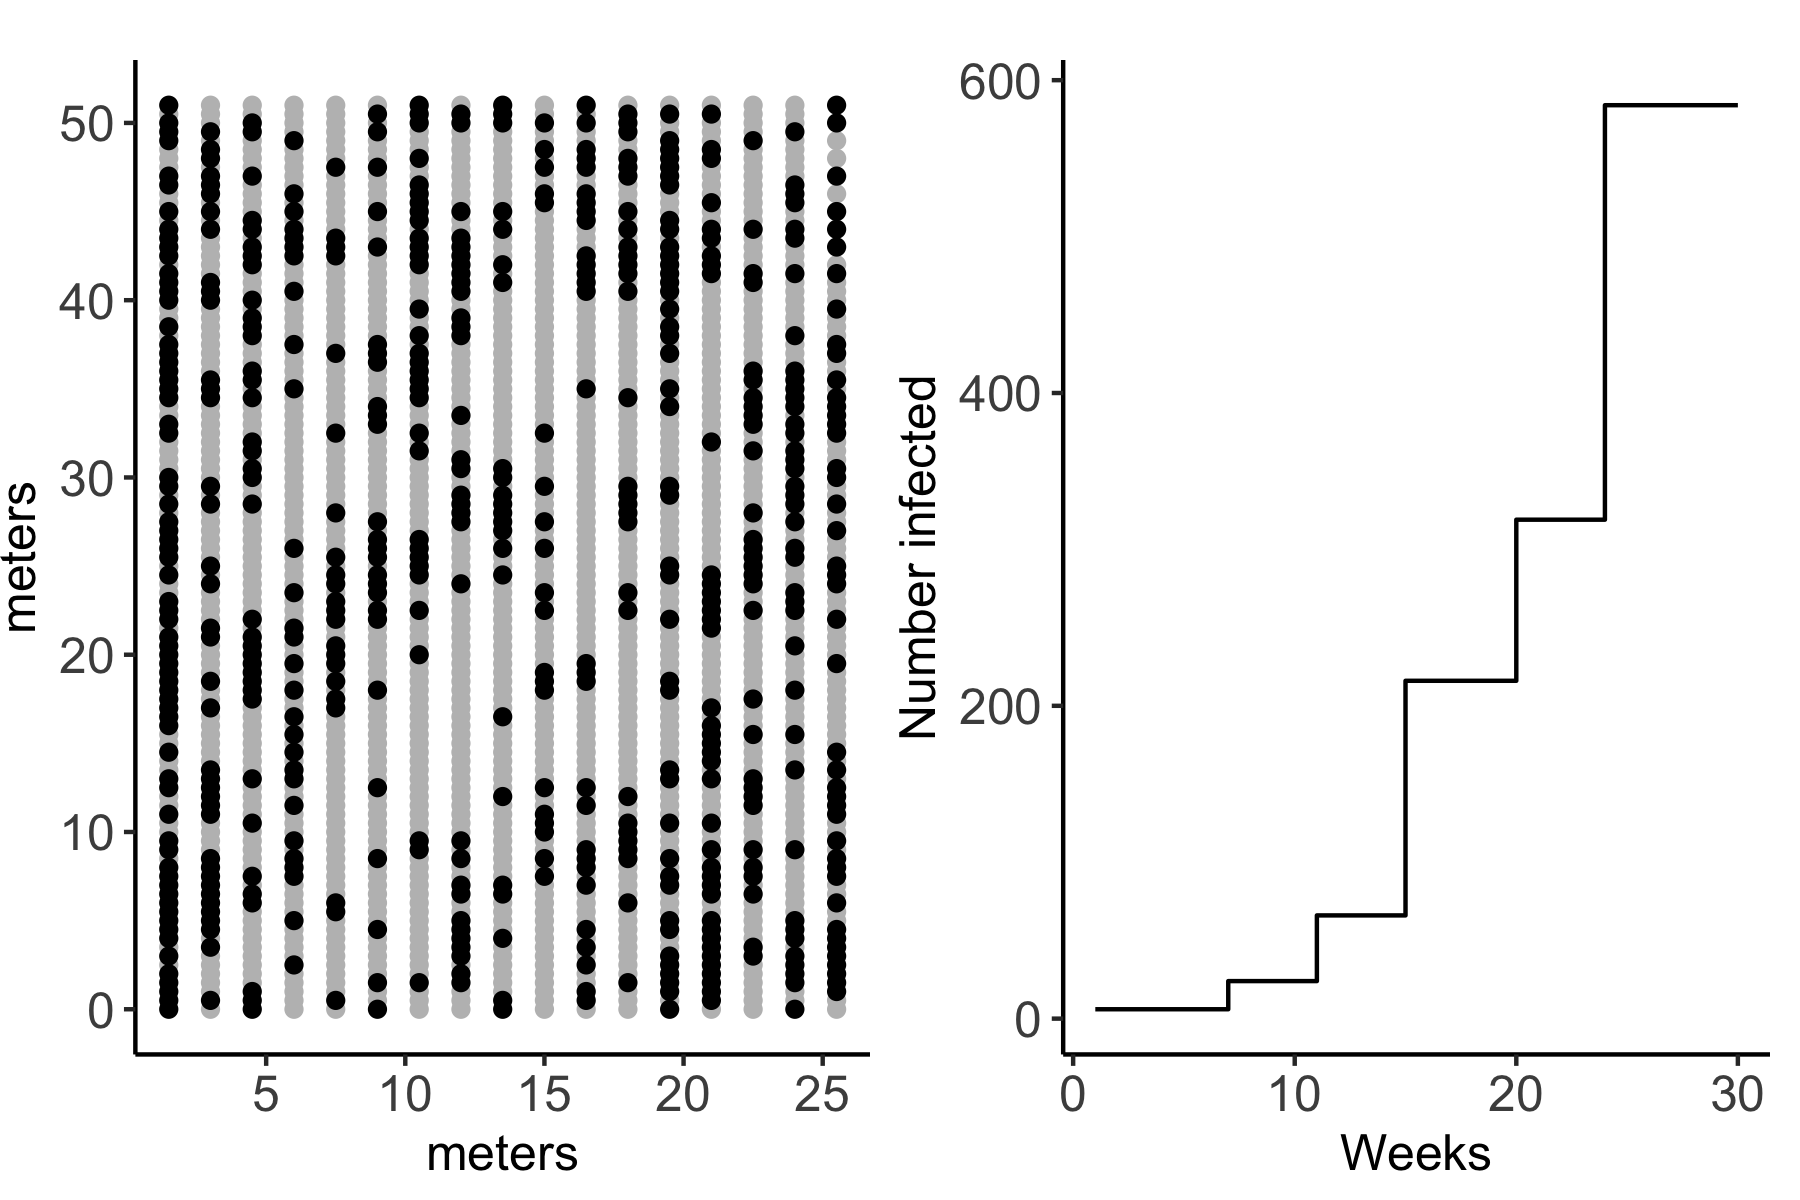
\includegraphics[height=0.45\linewidth, keepaspectratio]{/Users/nwelch/prelim/report/figures/figure_1.png}
\caption{Replicated Figure 1}
   \label{fig:data_plot}
\end{figure}

Figure \ref{fig:data_plot} summarizes the sugar cane data set. The black dots indicate locations of infected plants at the conclusion of the 30 week study period. Grey dots indicate the location of plants that were not infected. The plot on the right shows the cumulative number of infected plants for each inspection. 

\section{Methods}

\section{Results}

\section{Discussion}

\bibliography{/Users/nwelch/prelim/report/prelim_references}

\end{document}









